\section{Experimental Design}
We are providing experimental design for in lab or in simulation environment. In simulation environment, we provide modified protocol to fit simulation environment. 

\subsection{In Lab procedure}
\begin{itemize}
    \item Human participants will be shown a 2D empty work space with the goal marked clearly. Once they have a general idea of work space, their hand will then be placed at the starting point, and then they will be blindfolded.
    \item Then work space will be populated with obstacles.
    \item The experiment will begin by asking the person to move their hand towards the goal while keeping it close to the work space surface.
    \item In the first run, the Sawyer manipulator will guide the human using the continuous kinesthetic guidance system.
    \item In the second run the human will be able to move freely through the work space, and the robot will provide an on-demand kinesthetic guidance system when needed. If the participant hand enters the collision zone, a technician would voice alert (indicated through the warning node) and the robot will guide the human out of the collision zone to a point in space where participant can continue to navigate to the goal.
\end{itemize}
\subsection{In Simulation Environment}
\begin{itemize}
    \item We expect humans to act accordingly in simulation. 
    \item Give a human arm coordinates near obstacles. 
    \item Feed it to the motion planner.
    \item Check what trajectory robot comes with to avoid the collision.
\end{itemize}

\subsection{Changes to System Components}
Due to the unforeseen campus closure, a lot of the technical components that were a part of this project (refer to Figure \ref{fig:TechnicalComponents}) could not be actualised. 
For instance, the `Hand tracker component', the `Workspace Map' and `Sawyer Manipulator' were either omitted, integrated into other components, or replaced with a simulated system.

Since we are no longer tracking a live human hand, the `Hand Tracker' component was omitted and instead the position was published manually. 
This is because we cannot test the algorithm's effectiveness in conjunction with a human, and instead are focusing only on the effectiveness of the motion planner. 
The `Workspace Map' was integrated into the motion planner and free-navigation interrupter, by hardcoding the obstacle positions and dimensions. 
This is since we are not using an RBG camera to monitor the workspace.  
The `Sawyer manipulator' was replaced with a Gazebo simulator. 
It does not have any function other than displaying the output from the motion planner.
\begin{figure}[H]
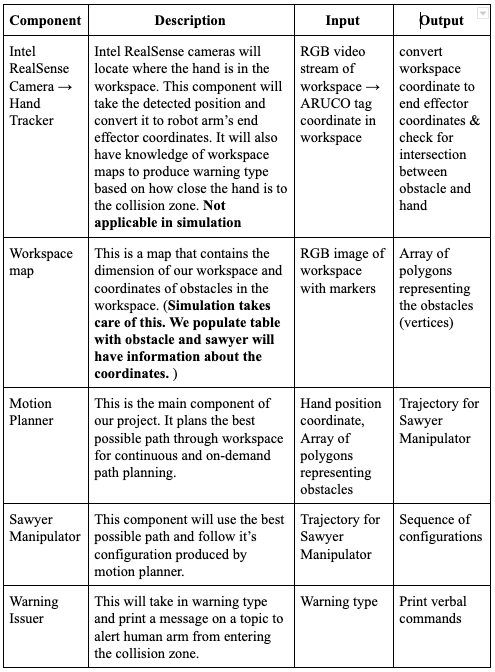
\includegraphics[width=\linewidth]{img/techcomponent.png}
\caption{Technical Components}
\label{fig:TechnicalComponents}
\end{figure}
